\subsection{XAI-Methoden für neuronale Netze}
Idee: zur Strukturierung:
Modell-Agnostische Methoden (hier jeweils angeben, ob es sich um eine Post-Hoc-Methode oder lokale oder globale handelt)
Modell spezifische Methoden (hier ein Kapitel je Algorithmus, z.B. CNN, LSTM, usw.)
Global Surrogate
Visualisierung 
Features
Instanzen
Sensitivität


Algorithmen:
Lime wird genutzt von \cite{weitz2019you} während sie Agenten mit menschlichen Zügen einsetzen, um Ekrlärungen darzulegen.
\cite{goldenfein2019algorithmic}: nennt Lime auch

Visualisierung \cite{zhou20182d}:
- Visualisierung für Naive Bayes [Becker, et al.: Visualizing the simple bayesian classifier; Kulesza et al.: Whyoriented
end-user debugging of naive bayes text classification]
- Visualisierung für Entscheidungsbäume [Baehrens et al.: How to
explain individual classification decisions] : 
- Visualisierung für SVM [Caragea et al.: Gaining insights into support vector machine pattern
classifiers using projection-based tour methods]
- Visualisierung für Hidden Markov Models [Dai und Cheng: HMMEditor: a visual editing tool for profile hidden Markov model]:


Mit Visualisierung könnte mna nicht nur Algorithmen Visualiseren, sondern auch Abhängigleiten zwischen den verschiedenen Ebenen der Pipeline, wie Deployment und Vorbereitung \cite{zhou20182d}
Manchmal bei komplexen Problemen wird auch Visualisierung zu komplex, man sollte immer Bezug zum Problem der Domäne haben \cite{zhou20182d}


Statistische Methoden \cite{zhou20182d}

Hyper-Fokus auf algorithmische Erklärungen von ML\cite{zhou20182d}
Feature/Instance Contributions: Was trägt ein Feature bei?
- Robnik-Sikonja et al. [Quality of classification explanations with PRBF.]: Beitrag von (Gruppen von Features) berechnen, indem man simuliert was passieren würde, sollten die Features fehlen
- Beiträge von einzelnen Instanzen: Landecker et al. [Interpreting individual classifications of hierarchical networks.] Contribution Propagation: Was trägt einzelne Instanz zu Netzwerk-Klassifikation bei? UND Baehrens et al. [How to
explain individual classification decisions.] local gradients, um zu beschreiben, wie eine Instanz verschoben werden muss, um ihr vorhergesagtes Label zu ändern, um einzelne Klassifizierungsentscheidungen zu erklären. 

Mathematische Modelle \cite{zhou20182d} um zu erklären, warum bestimmte Ergebnisse erzielt werden
- Chen et al. [Enhancing transparency and control when
drawing data-driven inferences about individuals]: statistisches Modell, das erklärt, warum in Social Media Rückschlüsse auf bestimmte Personen gezogen werden
- Zahavy et al. [Graying the black box: UnderstandingDQNs[cs]] und Zrihem et al. [Visualizing dynamics: from t-SNE to SEMI-MDPs]: Deep Q-Network
- Koh und Liang [Understanding black-box predictions via influence functions]: Influencefunctions um Modellvorhersage zurück zu den Trainingsdaten hin zu verfolgen

\cite{zhou20182d} sagt die beiden Methddoen (Feture/Instance Contributions und mathematische Modelle) wenden sich eher an ML-Experten --> Fokus nur auf die Entwicklung, Nutzer würde das eher verwirren als helfen

Model-agnostic-Methoden \cite{tsiakmaki2021case}:
- LIME ["" Why should i trust you?" Explaining the predictions of any classifier"]
- DLIME [DLIME: A Deterministic Local Interpretable Model-Agnostic Explanations Approach for Computer-
Aided Diagnosis Systems]
- SHAP [A Unified Approach to Interpreting Model Predictions]
- Anchors [Anchors: High-precision model-agnostic explanations]
- Counterfactual Explanations ["Interpretable counterfactual
explanations guided by prototypes, Counterfactual explanations without opening the black box: Automated decisions and the GDPR] --> hierfür hat Van Looveren et al. [Interpretable counterfactual explanations guided by prototype] noch eine Technik gemacht, mit der man die schneller generieren kann 

Einfache Modelle nehmen, die in sich verständlich sind und hierfür nur einfache Visualisierung erforderlich ist (wenn überhaupt) \cite{vaughan2020human}
- GAMS (Lou et al., 2012, 2013; Caruana et al., 2015). --> GAM für Experten

Post-Hoc-Erklärungen \cite{vaughan2020human}:
- LIME (siehe auch \cite{schoeffer2022human})
- SHAP - für Experten (siehe auch \cite{schoeffer2022human})
- TCAV (testing with concept activation vectors): Technik, die die Empfindlichkeit einer Vorhersage für ein übergeordnetes Konzept ausgibt (z. B. ob ein Objekt in einem Bild "gestreift" ist), das aus vom Benutzer bereitgestellten Beispielen gelernt wird (Kim et al., 2018).
- Koh und Liang [Understanding black-box predictions via influence functions]: Einflussreichste Trainingsdatenpunkte
- Counterfactuals: Wie muss ein Datenpunkt geändert werden, sodass er andere Vorhersage bekommt? (Russell, 2019;Weld and Bansal, 2019; Ustun et al., 2019;Wachter et al., 2018)

Die meisten Post-Hoc-erklärungen generieren lokale Erklärungen und kein globales, reflektieren somit also nciht die wahre Funktionsweise des Modells \cite{vaughan2020human} --> sagt sie liefern eher Beweise als wirklich Gründe zu liefern
Es gibt Ansätze, in denen Wissenschaftler hybride Modelle Entwickeln, die komplex sind, aber insofern in ihrer Komplexität begrenzt werden, als dass sie noch erklärbare VOrhersagen liefern (Lei et al., 2016: Rationalizing neural predictions; Alvarez-Melis and Jaakkola, 2018b: Towards robust interpretability with selfexplaining neural networks.).

\cite{hasib2022machine}: Beispiel für Nutzung von Lime für Log. Regression, KNN, SVM, XGBoost, Bayes

\cite{rajabiyazdi2020machine} STMLSTM-Erklärbarkeit mit:  LSTMVis [LSTMVis: A Tool for Visual Analysis of Hidden State Dynamics in Recurrent Neural Networks] 

\cite{chen2021novel}: visualization, sensitivity analysis, adversary attack
Feature Importance (Methode saliency Mask), Bedingungen visualisieren

\cite{chen2021novel}: A Novel Explainable Deep Belief Network Framework und ihre Anwendung für Feature Importance-Analyse: -> wenden zuerst Sensitivity Analyse an --> Sonferfall für Deep Belief Networks

\cite{tjoa2020survey} haben Literaturrecherche über XAI-Methoden gemacht im Kontext von Medizin
Sie unterteilen XAI-Methoden einmal nach Perceptive Interpretability und Interpretierbarkeit durch mathematische Struktur
Perceptive Interpretability:
Dekomposition (Saliency):
- CAM with global average pooling [42, 91]
Sonderformen: Grad-CAM [43], Guided Grad-CAM mit Feature Occlusion [68], Repsond CAM [44], Multi Layer CAM [92]
- LRP [13, 53]
Sonderformen: Bildklassifikation [45], Audiklassifikation- AudioMINST [47], LRP auf DeepLight [48], LRP auf CNN und BoW [49], LRP on compressed domain action recognition algorithm [50], LRP auf Video DL [52], BiLRP [57]
-DeepLIFT [57]
-Prediction Difference Analysis [58]
-Slot Activation Vectors [41]
- PRM (Peak Response Mapping) [59]
Sensitivität (Saliency):
-LIME
Sonderformen: MUSE with Lime [85], Guidelinebased Additive eXplanation (Optimierung von Komplexität, ähnlich wie Lime) [93]
Anders (Saliency):
- direct output labels - Training von NN mit multiple instance learning [65]
- Image Corruption and Testing Region of interest statistically [66]
- Attention map with autofocus convolutional layer [67]

Inversion (Signal):
-DecnovNet [72]
- Inverting representation with natural image prior [73]
- inversion using CNN [77]
- Guided Backpropagation [75,91]
Optimierung (Signal)
-Activation maximation/optimization [38]
Sonderformen: Activation maximation on Deep Belief Network [76], Activation maximation, multifacted feature visualization [77]
- Visualisierung durch regularized optimization [78]
- Semantic dictionary [79]
Andere (Signal):
- Network dissection [36, 37]

Verbal:
-Entscheidungsbäume
- Propositional logic, rule-based [82]
- Sparse Decision lisz [83]
- encoder-generator framework [86]
- Filer attribute probability density function [87]
- MUSE (Model understanding durch Subspace Explanations) [85]

mathematische Struktur
Vordefinierte Modelle:
-linear probe [101]
- Regression basiert auf CNN [106]
-Backwars model fpr interpretability of linear models [107]
-GDM [100]
-ProtoAttend [105]
verschiedene Kontextspezifische (Medizin) Modelle [131,132,133,134]

Korrelation (Feature Extraktion):
- PCA (Principal Component Analysis)
- SVD (Singular Value Decomposition)
- CCA (Canonical Correlation Analysis) [113]
- SVCCA (Singular Vector Canonical Correlation Analysis) [97] (Kombination von CCA und SVD)
F-SVD (Frame Singular Value Decomposition) [114]
- DWT (Discrete Wavelet Transform) + neuronale etzwerke [135]
- MODWPT (Maximal Overlap Discrete Package Transform) [136]
- GAN-basiertes Multi-Stage PCA [118]
-Estimating probability density with deep feature embedding [119]
Clustering (Feature Extraction):
- t-SNE (t-distributed stochastic neighbour embedding [77]
Sonderformen: t-SNE mit CNN [], Activation Atlas on GoogleNet [121], on latent space in meta-material design [122], on genetig data [137], mm-t-SNE on phenotype grouping [138]
- Laplacian Eigenmaps Visualition for Deep Generative Model [124]
- KNN on multi-center low-rank rep learning [125]
- KNN with triplet loss and query-result activation map pai  [139]
- Group-based interpretable NN with RW-based graph convolutional layer [123]

Sensitivität:
- TCAV (Testing with Concept Activation Vetors) [96]
Sonderformen: RVV [140], Concept Vectors mit USB [141], ACE [56]
- Influence Functions helfen adversial trainingspoints zu verstehen [129]
- Representer Theorem [130]
- SocRat (Structured-output Causual Rationalize) [127]
- Meta-predictors [126]
- Explanation Vector [128]

Andere:
- CNN mit sperable model[12]
-informationstheoretisch: information Bottleneck [98, 199]

Andere Perspektiven
Datengetrieben:
- Database of Method vs. Interpetierbarkeit [10]
- Case-Based Reasoning [143]
Invariance:
- integrated gradients [69, 94]
-Input invariance [71]
Utilities:
- Application based [144,145]
- Human based [146,147]
- Function based [2,5,42,43,44,45,96,97,144,145]

Erklärung der verschiedenen Kategorien \cite{tjoa2020survey}:
- Perceptice (wahrnehmbare) Interpretierbarkeit: können von Menschen wahrgenommen werden und sind "offensichtlich" - auf Bildern werden die zu klassifiziernenden Gegenständen gezeigt, Nachteile: eigentlicher Algorithmus bleibt Blackbox, Hintergrundobjekte werden nicht miteinbezogen
- Saliency Decomposition: Zerlegung der Signale, die innerhalb ihres Algorithmus propagiert werden, und Neuanordnung um interpretierbare Informationen zu liefern 
-Grenzen Saliency: Formulas nur heuristisch, interpretierbareer Beweis nicht nutzbar für Weiterenwicklung der Algorithmen
- Nachteile (von CAM, LRP): Gewichte und Aktivierung werden beachtet, Zwischenprozesse nicht
- Signalmethoden: Stimulierung von Neuronen anziegen --> Feature Maps, CNN
-Grenzen von Signalmethoden: decken Black-Box teilweise auf, Wie kann man extrahierte Signale weiter nutzen? Sind die Signale einzigartig oder zu gewissen Teilen konsistent?
-Verbale Interpretierbarkeit: für Menschen natürlicher zu erfassen, z.B. Sätze, die auf Kausalität hinweisen
- grenzen verbaler Itnerpretierbarkeit: Algorithmus bleibt Blackbox, nur Erklärungen sind interpretierbar, die Generierung derer bleibt Blackbox
- Mathematische Strukturen: um die Mechanismen von ML- und NN-Algorithmen aufzudecken
- Feature Extraktion: Welche Features sind am wichtigsten für die Klassifikation in eine bestimmte Klasse z.B.
- Grenzen Feature Extraction: Beweis bleibt mathematisches Artefakt, Mechanismen schwer zu beweisen
-Sensitivität: Methoden, die sich auf Lokalisierung, Gradients und Pertubationen stützen und schauen, wie "empfindlich" Modell ist
-Grenzen Sensitivität: Globale Sicht, Bildverarbeitung (Warum verändert kleine Änderung im Input Feature)

XAI-Methoden nach \cite{hanif2021survey}
Model-Agnostic: 
- Visualisierungsmethoden: PDP: Einfluss von Features, ICE: Einfluss von Änderungen von Features, ALE: Einfluss von Features
- Feature Interaction basiert: 
 1) Interaktion von Merkmalen unterinander Berechnung interagieren die Merkmale miteinander. Nach [22] wird die Interaktion zwischen zwei Merkmalen berechnet, indem die Differenz zwischen der partiellen Abhängigkeitsfunktion für diese beiden Merkmale zusammen und der Summe der partiellen Abhängigkeitsfunktionen für jedes einzelne Merkmal berechnet wird. Diese Methode hat den Nachteil, dass sie rechenintensiv ist. 
 2) Merkmalsrelevanz: Die Merkmalsrelevanz nimmt zu, wenn die Werte des Merkmals permutiert werden, um die echte Beziehung zwischen dem Merkmal und dem wahren Ergebnis zu stören. Wenn die Fehler nach der Neuanordnung der Merkmalswerte zunehmen, wird die Relevanz des Merkmals betont. Die Relevanz eines Merkmals gibt einen prägnanten und globalen Überblick über das Verhalten des ML-Modells. Die Tatsache, dass die Merkmalsbedeutung sowohl den Haupteffekt des Merkmals als auch die Interaktion berücksichtigt, ist nachteilig, da die Merkmalsinteraktion in die Bedeutung der zugehörigen Merkmale einbezogen wird. Kurz gesagt, das Vorhandensein einer Merkmalsinteraktion führt nicht dazu, dass die Bedeutung eines Merkmals zu einem Leistungsabfall führt. Darüber hinaus wird die Trainings- und Testmenge für die Merkmalsbedeutung verwendet, da sie die iterative Variation in der gemischten Datenmenge widerspiegelt. Es ist auch bemerkenswert, dass die Merkmalsbedeutung in den globalen Methoden enthalten ist.
- Global Surrogate: White-Box-Modell trainieren, sodass es sich an Ergebnisse des Blackbox-modells annähert
- Local Surrogate: spezifische Vorhersagen --> LIME, shapley Values, SHAP
- Instance-based:  Erklärungen für spezifische Beispiele des Systems statt für das Gesamtsystem erstellen um Rechenpower zu sparen --> nicht unbedingt Erklärung des Modells, sondern eher spezifische Beispiele 
1) Break Down: Diese Kategorie von Modellen liefert lokale Erklärungen und ist mit dem Algorithmus für partielle Abhängigkeiten verbunden, der einen schrittweisen Ansatz verwendet, der als "Break Down" bekannt ist. Dabei handelt es sich um ein iteratives Verfahren zur Identifizierung von Merkmalen, die einen Einfluss auf die Gesamtantwort haben. Wie im spieltheoretischen Ansatz dargelegt, wird mit einem Null-Team begonnen und auf der Grundlage der Beiträge der Beteiligten werden die Merkmalswerte nach und nach aufgefüllt. 
2) Kontrafaktisch: Nach Islam et al. [22] charakterisiert eine kontrafaktische Erklärung ein kausales Szenario als "Wenn X nicht eingetreten wäre, wäre Y nicht eingetreten". 
3) Adversarial: Die meisten Ansätze schlagen vor, den Abstand zwischen dem antagonistischen Beispiel und der zu kontrollierenden Instanz zu verringern und gleichzeitig die Prognose an das gewünschte Ergebnis des Systems anzupassen. Diese Methode ermöglicht eine Diagnose
4) Merkmalsauswahl: Zu den anderen vorgeschlagenen Strategien gehört die instanzbasierte Merkmalsauswahl, bei der die Merkmale in Abhängigkeit von der jeweiligen Instanz ausgewählt werden. 
knowledge-Based Techiken: Einbeziehen von Informationen (z. B. Fachwissen und/oder Korpuswissen zur Erklärung des Systems) und Domänenwissen: Wissensgraphen, um das Verständnis des Systems zu erzeugen. In dieser Studie wird behauptet, dass Wissensgraphen einen Weg zur Generierung von Erklärungen darstellen. [28]

Übersicht von \cite{hanif2021survey}, die sagt wofür was ist und auch an wen sich das am besten richten sollte, was wichtig ist für RQ3:
\begin{figure}
    \centering
    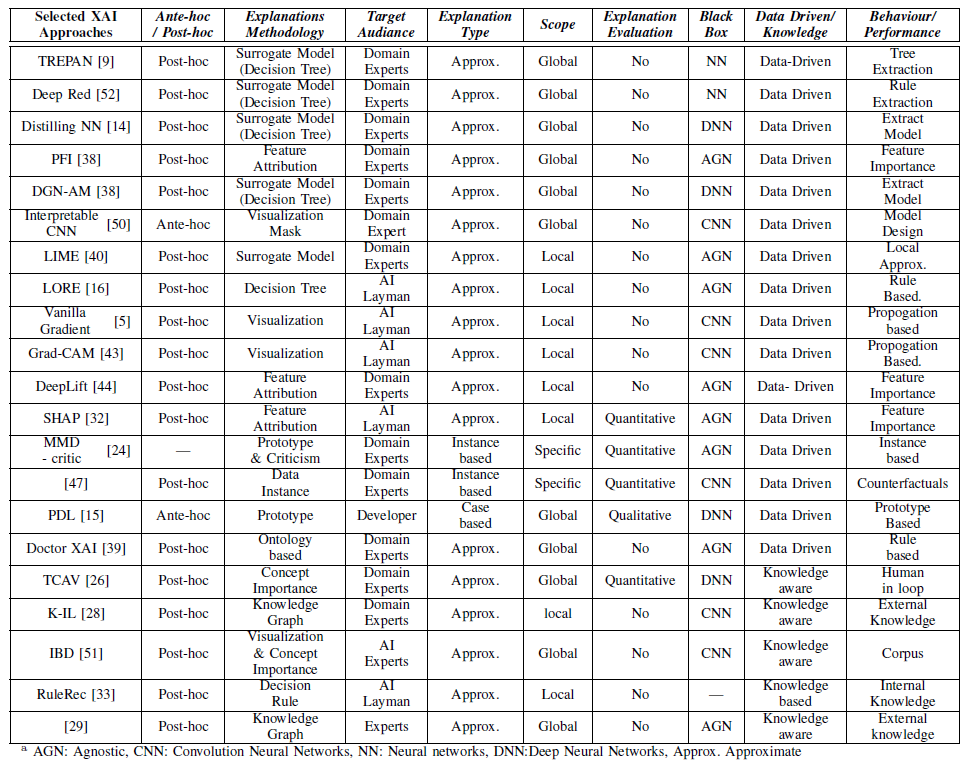
\includegraphics[scale=0.45]{pic/MA-Bilder/Literaturrecherche/21-XAI-Methoden mit Audience.PNG}
    \caption{Übersicht XAI-Methode mit Audience, entommen aus: \cite{hanif2021survey}}
    \label{Fig:XAI-MethodenmitAudience}
\end{figure}


Extraktion von Regeln aus einem neuronalen Netz heraus: \cite{de2015active} haben eine Technik entwickelt, die sich auf alle Black-Box-Modelle anwenden lässt, eine Regel sieht ungefähr so aus: Wenn (Gender = Male), Dann (das und das)
Grundsätzlicher Ansatz des Papers: - eigener Algorithmus für Regeln: ALPA -Idee: zur Verbesserung eines Regelsatzes in Bezug auf Genauigkeitein Whitebox trainieren, um Ausgabe eines komplexeren Blackbox-Modells nachzuahmen, das bessere Leistungen erbringt Bei Trainingssatz und einer Black-Box-Technik lässt sich Ähnlichkeit zwischen der Black-Box und der White-Box verbessern, indem dem White-Box-Algorithmus die vorhergesagten Zielwerte des Trainingssatzes anstelle der ursprünglichen, mit dem Trainingssatz verbundenen Zielwerte vorlegen  So wird die Blackbox zu einem Orakel für die Whitebox, und wir bezeichnen die mit den Vorhersagen dieser Blackbox verknüpften Trainingsdaten als Orakelsatz (im Gegensatz zum ursprünglichen Satz)
Es gibt noch andere Regeln-Extraktionen, hier sind ein paar Methoden
\begin{figure}
    \centering
    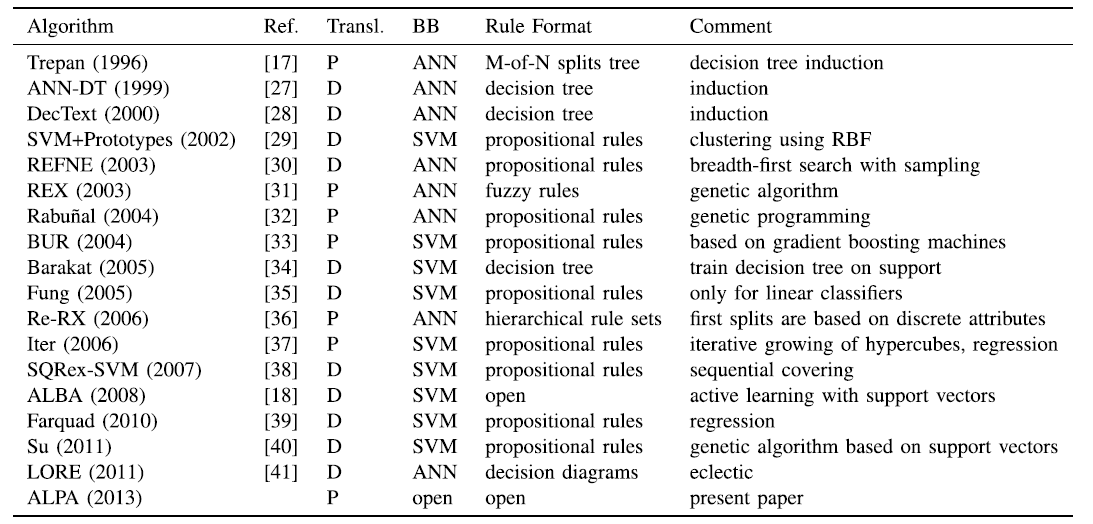
\includegraphics[scale=0.45]{pic/MA-Bilder/Literaturrecherche/27-RegelalgorithmenSurvey.PNG}
    \caption{Regelextraktion, entommen aus: \cite{de2015active}}
    \label{Fig:RegelextraktionAlg}
\end{figure}

Neuronale Netze: Neural Shrubs von \cite{caudle2019advanced} sind Entscheidungsbäume um neuronale Netze zu interpretieren (nutzbar für Regression und Klassifikation)
- gibt Ansätze wo Neuronalen Netze an den Blättern der Bäume sind [Decision tree–based classifier combined with neural-based predictor for water-stage forecasts in a river basin during typhoons: a case study in taiwan]

Visualisierungstool Advice (AdViCE: Aggregated Visual Counterfactual Explanations for Machine Learning Model Validation) nach \cite{gomez2021advice}:
- 3 Bestandteile: UI, Conterfactual Explanations, Debugging Workflow
- Counterfactual Explanations nach Martens [21] mit Erweiterung für tabellarische Daten
- so sieht es aus (1 main visualization,  2 filtering section,  3 model prediction range selector, 4 confusion matrix,  5 feature range selector,  6 feature sub-column,  7 information toggles,  8 median value,  9 histogram bin,  10 set of counterfactual explanations,  11 sorting method):
\begin{figure}
    \centering
    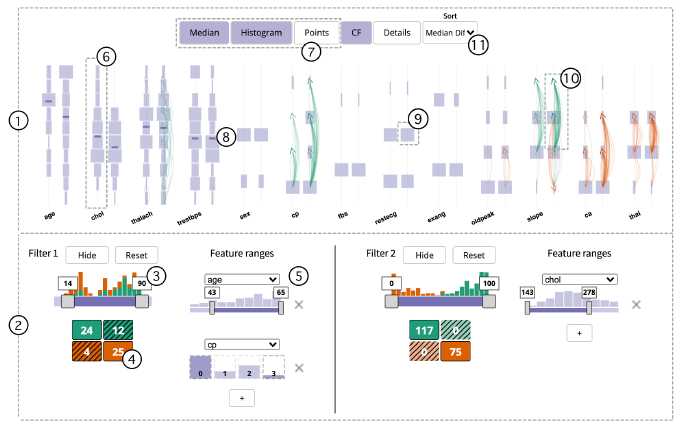
\includegraphics[scale=0.45]{pic/MA-Bilder/Literaturrecherche/29-UI.PNG}
    \caption{Advice Übersicht : \cite{gomez2021advice}}
    \label{Fig:Advice}
\end{figure}
- durch Interaktivität mittels Slider, Filtern und Klicken erhält Nutzer Infos zu Modellvorhersage, Korrektheit, Datenmerkmale
- man kann Daten/Erklärungen miteinander vergleichen
-Vorteile für Modellentwicklung und -validierung 
- Nachteile: Skalierbarkeit, Erklärungen für gesamte Datensätze aufwendig, viele Features schwer darstellbar, keine Bilder

genannte andere XAI-Methoden von \cite{gomez2021advice}:
-Black-Box-Erklärungen: LIME, SHAP, Anchor, LORE [10]
- Counterfactual Explanations generieren: Wachter et al[33], Ustun et al [32], DiCE[25], Martens [21]
- Visualisierung von Counterfactual Explanations: WIT (What-if-tol) [34], Seq2Seq [30], Rivelo (für Textklassifikation), Krause, ViCE [9], DECE [4]

\cite{de2018algorithmic}: post-hoc-Methode, die Modell als Black-Box betrachtet: Quantitative Influence Measures: \cite{datta2016algorithmic} und für SVM: Barbella et al. (2009, Understanding support vector machine classifications via a recommender system-like approach.)

\cite{goldenfein2019algorithmic}: Merkmale und deren Gewichte darstellen

Quantitative Input Influence (Messung des Einflusses von Input auf den Output) von \cite{datta2016algorithmic}:
- sowohl einzelne Instanzen als auch grundsätzlich für gesamte Gruppen
- Ergebnis eine (eher komplizierteren Rechnung\todo[inline]{hier noch genauer eingehen?}) sind dann Reports die sagen, welches Feature am meisten Einfluss hatt, oder persönhliche Report (z.B. warum Person X negativ klassifiziert wurde mit Angabe ihrer Features)
- Grenzen des Ansatzes: Grenzen: schwer zu verstehende Inputs, Bilder, Sprache, Videos

\cite{blacklaws2018algorithms}: Methode "Code veröffentlichen" bringt nicht, denn wir sehen durch Code nciht, wie Alg. funktioniert, da er sein Wissen aus Daten zieht

\cite{wang2020explainable} machen XAI im Umfeld des intrusion detection systems - hier nutzen sie SHAP für globale und lokale Erklärungen
- sie nennen sonst noch LRP und LEMMNA als andere Methoden
- SHAPLEY-Wert: Beitrag eines Merkmalswertes zur Vorhersage
- SHAP (SHAPLEY ADDITIVE EXPLANATIONS): erklärt die Vorhersage einer Instanz x, indem es den Beitrag jedes Merkmals zur Vorhersage berechnet
- Unterschied von LIME und SHAP: Der große Unterschied zu LIME ist die Gewichtung der Instanzen im Regressionsmodell. LIME gewichtet die Instanzen danach, wie nahe sie der ursprünglichen Instanz sind. Je mehr 1en im Koalitionsvektor, desto größer ist die Gewichtung in LIME. SHAP hingegen gewichtet die gesampelten Instanzen nach dem Gewicht, das die Koalition bei der Shapley-Wert-Schätzung erhalten würde.
- Vorteile SHAP: Erstens hat SHAP eine solide theoretische Grundlage in der Spieltheorie. Shapley-Werte sind die einzigen Lösungen, die drei Eigenschaften erfüllen: Symmetrie, Dummy und Additivität. SHAP kann diese Eigenschaften ebenfalls erfüllen, da es Shapley-Werte aus linearen Modellen erhält. Zweitens: SHAP verbindet LIME und Shapley-Werte. Es hilft, das Feld des interpretierbaren maschinellen Lernens zu vereinheitlichen. Schließlich bietet SHAP eine schnelle Berechnung für maschinelle Lernmodelle im Vergleich zur direkten Berechnung des Shapley-Wertes.
- sie zeigen einzelne Instanzen (lokal) und Kombination mehrer Instanzen (global)
- Beziehungen zwischen Merkmalen werden auch dargestellt: Zunächst wird der Wert des Merkmals in mehrere Intervalle unterteilt; dann werden die Shapley-Werte dieses Merkmals über die Daten hinweg berechnet. Schließlich werden die Shapley-Werte in jedem Intervall gemittelt. 



\cite{palaniyappan2022aqx}Feature Importance Visualisierung am Beispiel von  Vorhersage von Luftqualität:
- Feature Importance auf unterschiedlichen Ebenen visualisiert zusammen mit Informationen über Performance und Rohdaten
- Um globale Muster des Merkmalsbeitrags zu verstehen, zeigt die Übersicht (A) den Merkmalsbeitrag aggregiert und als tagesbezogene Übersicht (a1), stundenbezogene Übersicht (a2) und ortsbezogene Übersicht (a3) an. Sie hilft auch bei der Eingrenzung auf die Instanz, die von Interesse ist. 
- Die Leistungsansicht (B) zeigt und vergleicht die Vorhersagegenauigkeit der ML- und CMAQ-Modelle für Überwachungsstationen in der Ansicht "Mittlerer IOA (Index der Übereinstimmung)" (b1) und die vom Modell erfassten räumlichen Muster für die gesamte Region Hongkong in der Ansicht "Räumliche Karte" (b2) für den Zielzeitpunkt und den Schadstoff, um zu verstehen, was das Modell lernen kann und was nicht. Die Rohdatenansicht 
- (C) zeigt die Windtrajektorien für den eingegebenen Zeitraum anhand von Animationen, die helfen zu verstehen, wie der Wind Schadstoffe von einem Ort zum anderen trägt. 
-Die Ansicht "Feature-Temporal Importance" (D) zeigt den Gesamtbeitrag der eingegebenen Merkmale für die betreffende Instanz und hilft dabei, die Merkmale mit dem höchsten Beitrag für die Vorhersage zu erkennen. 
- Die räumlich-zeitliche Ansicht (E) zeigt den Beitrag von Gitterstandorten aus verschiedenen Zeitstempeln, was hilft, den Beitrag von Merkmalen aus verschiedenen räumlichen Standorten für den Eingabezeitraum zu verstehen.
- Feature Relevanz-Methoden: SHAP, PDP (Nachteil: Rechenaufwendig)
-Gradientenbasierte Methoden liefern Merkmalsrelevanz, indem sie die erste Ableitung der Ausgabe in Bezug auf die Eingabe berechnen [29].
- Visualisierung des Modellverhaltens besonders geeignet für Endnutzer, weil sie interaktiv damit was machen können
- für Feature Importance: first-derivative saliency [29]
- Grenzen: große Anzahl an Features schlecht abbildbar --> unübersichtlich

\cite{strobel2019aspects}:
- Monotone Influence Measures (vgl.: J Sliwinski, M Strobel, and Y Zick. 2019. Axiomatic Characterization of Data-Driven Influence Measures for Classification): Dies sind Funktionen, die bei einem Datensatz jedem Merkmal einen Wert zuweisen; dieser Wert sollte in etwa der Bedeutung des Merkmals bei der Beeinflussung des Klassifikationsergebnisses für einzelne Datenpunkte entsprechen. Einige Measures beziehen sich auf die geometrische Manipulation des Datensatzes, d. h. auf das Verhalten des Maßes bei Rotation oder Verschiebung der Daten; wir haben auch Axiome zur Kontinuität und eine Form der Monotonie berücksichtigt. Aus diesen Axiomen leiteten wir eine Klasse von Einflussmaßen ab, die wir als monotone Einflussmaße (MIM) bezeichneten und die diese Axiome eindeutig erfüllten.
-\cite{datta2016algorithmic}: Einflussmaß für Datensätze; in ihrer Arbeit wird Einfluss jedoch als globales Maß interpretiert 
- Eine andere Arbeit, die den Black-Box-Zugriff nutzt [LIME], verwendet Abfragen an den Klassifikator in einer lokalen Region in der Nähe des interessierenden Punktes, um den Einfluss zu messen. Adler et al. setzen den Einfluss eines bestimmten Merkmals mit der Fähigkeit gleich, den Wert von us den übrigen Merkmalen abzuleiten, nachdem es verdeckt wurde; diese Idee ist die Grundlage für einen Rahmen zur Überprüfung von Black-Box-Modellen auf der Grundlage statistischer Analysen. Dieser Ansatz setzt jedoch voraus, dass man Vorhersagen für einen Datensatz machen kann, bei dem einige Merkmale entfernt wurden.

\cite{pan2021automated}
- gradientenbasierte Methode [31] ist ein erfolgreicher Versuch, interpretierbares maschinelles Lernen zu ermöglichen. Sie berechnet eine bildspezifische Klassen-Salienzkarte, die dem Gradienten der Ausgangsneuronen entspricht. 
- Integrated Gradients [32] ist eine Variante der Saliency Map, bei der integrale Methoden zur Verbesserung der Informationsgewinnung eingesetzt werden. 
- Verschiedene erklärbare ML-Techniken [33]-[35] nutzen das Konzept der "Dekonvolution" zur Umkehrung und Visualisierung des Merkmalslernens in neuronalen Faltungsnetzen (CNNs). 
- DeepLIFT [36] ist ein weiterer beliebter Algorithmus, der entwickelt wurde, um die Aktivierungseffekte der einzelnen Neuronen zu beobachten und jedem von ihnen einen Beitrag zuzuweisen. - Wir verwenden die Methode der "Modell-Destillation" [37] als EML-Technik. Der Grundgedanke der Modelldestillation besteht darin, dass ein separates Modell entwickelt wird, das als "destilliertes Modell" bezeichnet wird und eine Annäherung an das Input-Output-Verhalten des Zielmodells für maschinelles Lernen darstellt. Dieses destillierte Modell ist inhärent erklärbar, was dem Benutzer hilft, die Entscheidungsregeln oder Eingabemerkmale zu identifizieren, die die endgültige Entscheidung beeinflussen, wie in Abbildung 3 dargestellt. Daher werden leichtgewichtige Strukturen bevorzugt, wie lineare Regression [38], Entscheidungsbaum [39] oder Objektgraph [40].

Neuronale Netze \cite{westin2020building}: ähnlicher Weise werden Erklärungen für tiefe neuronale Netze (DNNs), die für die Bilderkennung verwendet werden, oft entweder mit Hilfe der Salienzmaske, die Schlüsselbereiche/Merkmale im Eingabebild visualisiert, oder durch Aktivierungsmaximierung, die die Schlüsselneuronen in bestimmten Schichten bestimmt, die durch das Eingabebild aktiviert werden. 
Beispielhafte Methoden für die Bildklassifizierung mit Faltungsneuronalen Netzen (CNNs) sind die pixelweise Dekomposition (PWD), die Heatmaps verwendet, um einzelne Pixel des Eingabebildes zu visualisieren, die die Ausgabe bestimmen [36], und die Visual-Back-Prop-Methode (VBP), die Masken verwendet, um die Menge der Pixel im Eingabebild zu visualisieren, die die Ausgabe bestimmen [37].

\cite{westin2020building}:
- lokale interpretierbare modell-agnostische Erklärungen (LIME) [38]: Es hat sich jedoch gezeigt, dass einige von ihnen instabil sind (z. B. LIME), da sie unterschiedliche Erklärungen für ähnliche Eingaben liefern, was ihre Verwendung in Bereichen mit hohem Risiko verhindert [41] 
- kontextuelle Erklärungsnetzwerke [39]: Contextual Explanation Networks ist ein interessanter Ansatz für XAI, der ML-Methoden und probabilistische Modelle kombiniert [39]. Contextual Explanation Networks verarbeitet eine Teilmenge von Eingabemerkmalen und erzeugt Parameter für ein spärliches lineares Modell, das von Domänenexperten bewertet werden kann. Anschließend wird das generierte Modell auf eine weitere Teilmenge von Eingaben angewendet und erzeugt eine Vorhersage [39]. Den Entwicklern zufolge ist dieser Ansatz robust und ein Kandidat für Bereiche mit hohem Risiko.
- kontextuelle Dekomposition [40]: Contextual Decomposition [40] liefert Erklärungen durch die Zerlegung der LSTM-Ausgabe (Long Short Memory).

Kritik an dieser Übertragungsmethode: \cite{krause2017workflow}
 sind transparent, ABER schwer zu generalisieren und Anwensund dieser auf andere Modelle nciht transparent - geben nur ein begrenztes Bild dessen wieder, wie Modell funktioniert